%\documentclass[draft]{beamer}
\documentclass{beamer}
%%%%%%%%%%%%%%%%%%%%%%%%%%%%%%%%%%%%%%%%%%%%%%%%%%%%%%%%%%%%%%%%%%%%%%%%%%%%
\let\Tiny=\tiny
\usefonttheme[onlymath]{serif}
\usepackage{bm}
\usepackage{amsmath}
\usepackage{amssymb}
\usepackage{microtype}
\usepackage{booktabs}
%%% INCLUDE FILE FOR DEFINITIONS
%%% These may require various packages.

% Shortcuts in regular text
\newcommand{\degs}{\ensuremath{^\circ}}
\newcommand{\EE}[1]{\ensuremath{\times 10^{#1}}}
\newcommand{\ttimes}{\ensuremath{{}\times{}}}
\newcommand{\cclicense}{%
  \smash{\raisebox{-0.45ex}{%
  \setlength{\unitlength}{1em}%
  \begin{picture}(1,1)%
    \put(0.5,0.5){\circle{1}}
    \put(0.5,0.5){\hbox to 0pt{\hss\raisebox{-.45ex}{\tiny\textsf{CC}}\hss}}
  \end{picture}%
  }}%
  \hskip -1em%
  \href{http://creativecommons.org/licenses/by-nc-sa/3.0/}%
  {\ \hskip 1em \textsf{BY-NC-SA}}%
}

%\newcommand{\horizsep}{{\par\noindent\centering\rule[.25ex]{.75\columnwidth}{2pt}\par}}
\newcommand{\horizsep}{\vspace{\baselineskip}\noindent\hspace{\stretch{1}}$
\ast\qquad \ast\qquad \ast\qquad
$ \hspace{\stretch{1}} \vspace{\baselineskip}}
\newcommand{\pytrt}{\textsf{PyTRT}}

% Research
\newcommand{\lop}[1]{\mathcal{L}\!\left[#1\right]}
\newcommand{\lopinv}[2]{\mathcal{I}_{#1}\!\left[#2\right]}
\newcommand{\Dtens}{\mat{D}}
\newcommand{\Etens}{\mat{E}}
\newcommand{\Identitytens}{\mat{I}}
\newcommand{\APone}{AP$_1$}
\newcommand{\Pone}{P$_1$}
\newcommand{\SN}{S$_N$}%{S$_\text{N}$}%{$S_N$}%
\newcommand{\PN}{P$_N$}%{P$_\text{N}$}%{$P_N$}%
\newcommand{\CN}{Crank--Nicolson} %Yes, it's Nic not Nich
\newcommand{\Eddington}{\mathcal{E}} %whatever symbol I decided for Eddington
\newcommand{\RadEn}{E} %whatever symbol I decide for radiation energy
\newcommand{\Sigmatr}{\Sigma_{\mathit{tr}}}

% Program names
\newcommand{\cpp}{\textsf{C\raisebox{0.2ex}{++}}}

% General math shortcuts
\newcommand{\ud}{\mathop{}\!\mathrm{d}}
\newcommand{\pder}[2]{\frac{\partial #1}{\partial #2}}
\newcommand{\oder}[2]{\frac{\mathrm{d} #1}{\mathrm{d} #2}}
\newcommand{\tpder}[2]{{\partial #1}/{\partial #2}} %inlined
\newcommand{\toder}[2]{{\mathrm{d} #1}/{\mathrm{d} #2}} %inlined
\newcommand{\lra}{ \quad \Longrightarrow \quad }
\newcommand{\eexp}{\mathop{}\!\mathrm{e}} % upright ``e'' for exponent
\newcommand{\expp}[1]{\exp\!\left( {#1} \right)} % exp with parentheses
\newcommand{\qeq}{\stackrel{\mathrm{?}}{=}}

% Probability
\newcommand{\expectation}[1]{\mathop{}\!\mathrm{E}\!\left[ #1 \right]}
\DeclareMathOperator{\Var}{Var} % variance

% Asymptotic analysis
\DeclareMathOperator{\Ei}{Ei} % Exponential function
\newcommand{\lapl}[1]{\mathcal{L}[{#1}]} %laplace

%change the Re and Im operators from fancy curly letters
\DeclareMathOperator{\MathOpRe}{Re}
\renewcommand{\Re}{\MathOpRe}
\DeclareMathOperator{\MathOpIm}{Im}
\renewcommand{\Im}{\MathOpIm}

%imaginary ``i'' , upright 'i' or \imath
\newcommand{\iimag}{\mathrm{i}}

% Finite differences
\newcommand{\hot}{\text{h.o.t.}}
\newcommand{\inv}{^{-1}}

% Numerical Linear Algebra
\newcommand{\conj}{^{\ast}} % complex conjugate (transpose)
\newcommand{\norm}[1]{\left\| #1 \right\|} % double pipe
\newcommand{\abs}[1]{\left| #1 \right|} % single pipe
\newcommand{\eps}{\varepsilon}
\DeclareMathOperator{\fl}{fl}

\DeclareMathOperator{\acosh}{arccosh} 

% Define a command to write a nice-looking element, e.g. 4,2 He
\newcommand{\elem}[3]{\ensuremath{{}^{{#1}}_{{#2}}\mathrm{{#3}}}}

% Vector definitions
\newcommand{\mat}[1]{\mathbf{#1}} %matrix is bold upright
\renewcommand{\vec}[1]{\bm{#1}} %vector is bold italic
\newcommand{\op}[1]{\mathsf{#1}} % ``operator'' is sans serif

\newcommand{\vd}{\bm{\cdot}} % slightly bold vector dot
\newcommand{\del}{\vec{\nabla}} % gradient (Del) is bold
\newcommand{\grad}{\vec{\nabla}} % gradient

%\newcommand{\abr}[1]{\langle {#1} \rangle}
\newcommand{\abr}[1]{\left\langle {#1} \right\rangle} % angle brackets for avg.

%% topbox is useful in extended definitions of math terms inside an align
\newcommand{\topbox}[2][0.6]{\parbox[t]{#1\columnwidth}{\raggedright{}#2}}

% commands to make text in math mode appear as zero-width (better-looking
% integrals/sums, e.g.)
% from mathmode.pdf page 74, or Alexander R. Perlis ``A complement to \smash,
% \llap, and \rlap''

\def\mathllap{\mathpalette\mathllapinternal}
	\def\mathllapinternal#1#2{%
	\llap{$\mathsurround=0pt#1{#2}$}%
}
\def\clap#1{\hbox to 0pt{\hss#1\hss}}%
\def\mathclap{\mathpalette\mathclapinternal}%
\def\mathclapinternal#1#2{%
	\clap{$\mathsurround=0pt#1{#2}$}%
}
\def\mathrlap{\mathpalette\mathrlapinternal}%
\def\mathrlapinternal#1#2{%
	\rlap{$\mathsurround=0pt#1{#2}$}%
}

\setSRJthesisfigurepaths

\definecolor{lightgray}{gray}{0.85}
%%%%%%%%%%%%%%%%%%%%%%%%%%%%%%%%%%%%%%%%%%%%%%%%%%%%%%%%%%%%%%%%%%%%%%%%%%%%

%30 minute presentation
%15 minutes scheduled for questions
%1 hour allotted total

\usetheme{AnnArbor}
\usecolortheme{seahorse}
\usecolortheme{orchid}
\setbeamercolor*{frametitle}{use=structure,bg=structure.fg!20!white}
\setbeamercolor*{frametitle right}{use=structure,bg=structure.fg!20!white}
\setbeamertemplate{navigation symbols}{\insertframenavigationsymbol}
\setbeamertemplate{caption}[numbered]

\title[Flatland]%
{Diffusion Boundary Conditions in Flatland Geometry}

\author[SRJ, EWL]{Seth~R.~Johnson \and Edward~W.~Larsen}

\institute[UMich]{
University of Michigan, Ann Arbor
}
\date[10/31/2011]{October 31, 2011}

%\AtBeginSection[]
%{
%\begin{frame}
%  \frametitle{Outline}
%  \tableofcontents[currentsection]
%\end{frame}
%}

\hypersetup{colorlinks=true,linkcolor=black}

% only show section headings in table of contents
\setcounter{tocdepth}{1}

%use symbols for footnote
\renewcommand{\thefootnote}{\fnsymbol{footnote}}

\begin{document}
%%%%%%%%%%%%%%%%%%%%%%%%%%%%%%%%%%%%%%%%%%%%%%%%%%%%%%%%%%%%%%%%%%%%%%%%%%%%

\begin{frame}
\titlepage
\begin{center}
  
\includegraphics[width=0.2\textwidth]{umlogo}
\end{center}
\smash{
\includegraphics[width=0.2\textwidth]{neup-small}}
\end{frame}

%%%%%%%%%%%%%%%%%%%%%%%%%%%%%%%%%%%%%%%%%%%%%%%%%%%%%%%%%%%%%%%%%%%%%%%%%%%%
%\begin{frame}
%  \frametitle{Outline}
%  \tableofcontents
%\end{frame}
%%%%%%%%%%%%%%%%%%%%%%%%%%%%%%%%%%%%%%%%%%%%%%%%%%%%%%%%%%%%%%%%%%%%%%%%%%%%
\section{Introduction}
%%%%%%%%%%%%%%%%%%%%%%%%%%%%%%%%%%%%%%%%
\begin{frame}{What is flatland?}
  \begin{itemize}
    \item Fictional two-dimensional universe \cite{Abb1884} in which particles
      are constrained to exist and travel in a 2-D plane
    \item Multi-dimensional geometry with smaller phase space in angle
      \begin{itemize}
        \item Flatland: $(x,y,\omega)$; 2-D: $(x,y,\mu,\omega)$
        \item Polar cosine is set to zero
      \end{itemize}
    \item Useful testbed for methods development
      \begin{itemize}
        \item Smaller phase space means computationally cheaper
        \item Angle-dependent quantities are easier to visualize
      \end{itemize}
  \end{itemize}
\end{frame}

%%%%%%%%%%%%%%%%%%%%%%%%%%%%%%%%%%%%%%%%
\begin{frame}{Channel surfing}
\begin{center}
  How do you design a 2-D test problem to model radiation in a channel?
\end{center}
\vspace{-.75in}

\begin{minipage}[c]{2.25in}%
  \vspace{.75in}%
  \includegraphics<1-2>[width=2in]{chord-flatland}%
  \includegraphics<3>[width=2in]{channel-xy}%
\end{minipage}
\begin{minipage}[c]{2.25in}%
  \rule{0pt}{3in}%
  \includegraphics<2>[width=2in]{chord-xyz}%
  \includegraphics<3>[width=2in]{channel-xyz}%
\end{minipage}
\end{frame}

%%%%%%%%%%%%%%%%%%%%%%%%%%%%%%%%%%%%%%%%
\begin{frame}{Channel surfing}
\begin{center}
  How do you design a 2-D test problem to model radiation in a channel?
\end{center}
\vspace{-.75in}

\begin{minipage}[c]{2.25in}%
  \vspace{.75in}%
  \includegraphics<1-2>[width=2in]{chord-flatland}%
  \includegraphics<3>[width=2in]{channel-xy}%
\end{minipage}
\begin{minipage}[c]{2.25in}%
  \rule{0pt}{3in}%
  \includegraphics<2>[width=2in]{chord-xyz}%
  \includegraphics<3>[width=2in]{channel-xyz}%
\end{minipage}
\end{frame}

%%%%%%%%%%%%%%%%%%%%%%%%%%%%%%%%%%%%%%%%%%%%%%%%%%%%%%%%%%%%%%%%%%%%%%%%%%%%
\section{Theory}
\subsection{Theory}

%%%%%%%%%%%%%%%%%%%%%%%%%%%%%%%%%%%%%%%%
\section{Results}

%%%%%%%%%%%%%%%%%%%%%%%%%%%%%%%%%%%%%%%%%%%%%%%%%%%%%%%%%%%%%%%%%%%%%%%%%%%%
\section{Conclusions}
%%%%%%%%%%%%%%%%%%%%%%%%%%%%%%%%%%%%%%%%%%%%%%%%%%%%%%%%%%%%%%%%%%%%%%%%%%%%
\appendix
%%%%%%%%%%%%%%%%%%%%%%%%%%%%%%%%%%%%%%%%
\begin{frame}
  %\frametitle{Questions?}

{\par\centering%
  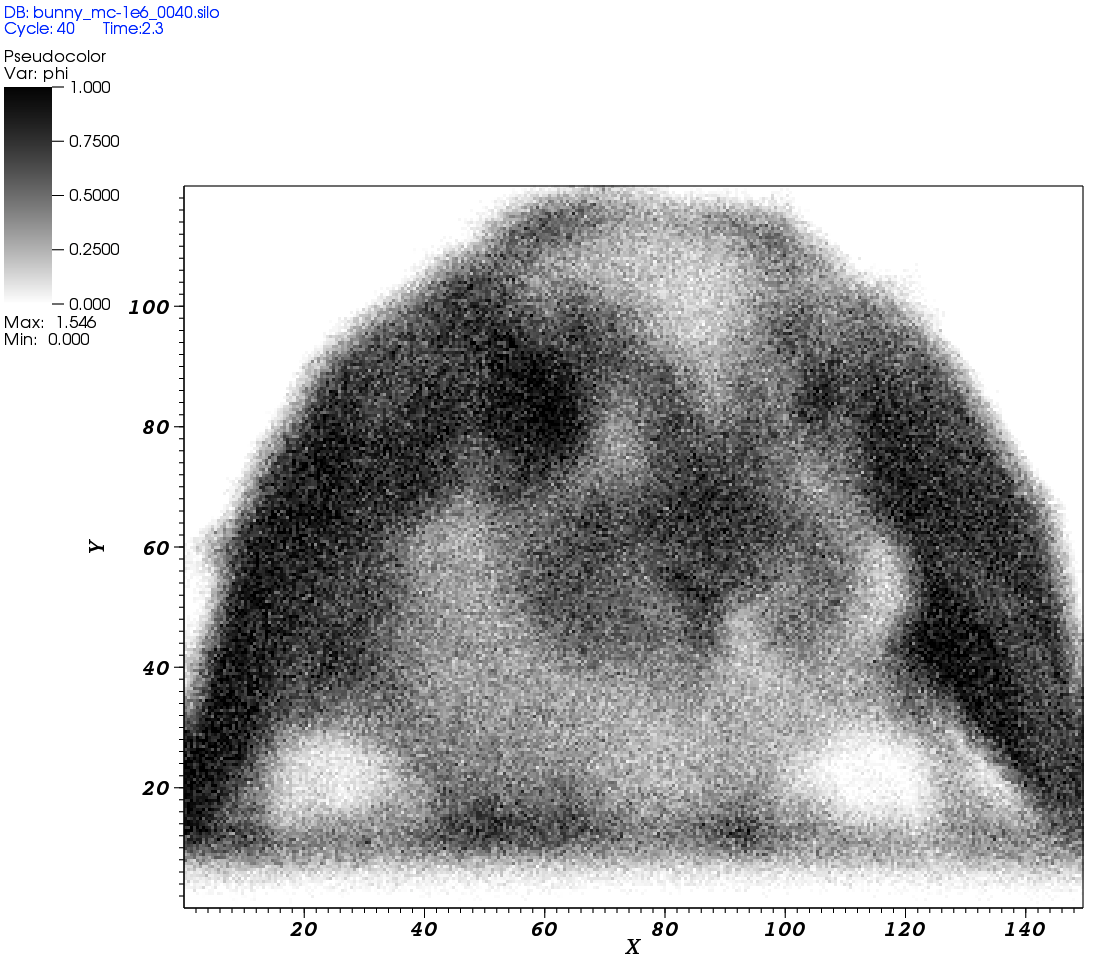
\includegraphics[height=2.75in]{bunny-transport}

}
{\setlength{\baselineskip}{-\baselineskip} \tiny 
This material is based upon work supported under a National Science Foundation
Graduate Research Fellowship and a Department of Energy Nuclear Energy
University Programs Graduate Fellowship. Any opinions, findings, conclusions or
recommendations expressed in this publication are those of the author and do
not necessarily reflect the views of the National Science Foundation or the
Department of Energy Office of Nuclear Energy.\par}
\end{frame}

%%%%%%%%%%%%%%%%%%%%%%%%%%%%%%%%%%%%%%%%
\begin{frame}
  \frametitle{References}
\bibliographystyle{ans}
\bibliography{../../SRJall}
\end{frame}
%%%%%%%%%%%%%%%%%%%%%%%%%%%%%%%%%%%%%%%%%%%%%%%%%%%%%%%%%%%%%%%%%%%%%%%%%%%
\end{document}

